%----------------------------------------------------------------------------   
\chapter{Használt eszközök bemutatása}
%---------------------------------------------------------------------------- 

\section{Kubernetes}

A Kubernetes egy nyílt forráskódú konténer kezelő platform, amivel automatizálni
lehet a legtöbb feladatot, ami a fejlesztés, karbantartás vagy skálázással 
kapcsolatos. A Google fejlesztette eredetileg, de jelenleg a Cloud Native
Computing Foundation - CNCF vette át a karbantartását. 

Kubernetes fürtöt létrehozhatunk lokálisan a saját szerveren is vagy felhőben,
ami lehet publikus, privát vagy hibrid hozzáférésű. Viszont azt figyelembe 
kell venni, hogy egy Kubernetes fürtöt nem egyszerű kiépíteni lokálisan, 
szóval ha nem szükséges, akkor lehet használni felhőszolgáltatók Kubernetes 
motorjai, mint az Amazon AKS, Linode LKE vagy a Google GKE szolgáltatása.
Ilyenkor egy teljes fürtöt, ami az általunk beállított paramétereket használja.

\subsection{Felépítése}

\begin{figure}[!ht]
	\centering
	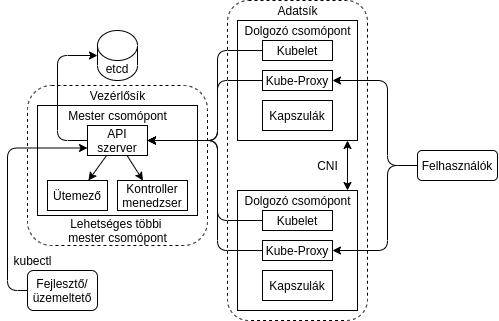
\includegraphics[width=1\textwidth, keepaspectratio]{figures/k8s_architecture.png}
	\caption{Kubernetes fürt felépítése}
	\label{fig:HVSpaces}
\end{figure}

Egy Kubernetes fürt kettő részből áll egy vezérlő- és egy adatsíkból, ahol a 
vezérlősíkban szereplő mester csomópontok tudják vezérleni az adatsíkban 
lévő dolgozó csomópontokat és a fejlesztők vagy üzemeltetők a mester által
hirdetett API-n keresztül képesek parancsokat kiadni. Míg a dolgozó 
csomópontokon futó alkalmazáshoz a felhasználók csak az általuk hirdetett 
Kube-Proxy segítségével tudnak hozzáférni. 

A kapcsolat mester és dolgozó között az API szerver és a Kubelet kommunikációján
alapul. Ha a fejlesztő szeretne egy új alkalmazást telepíteni a fürtön, akkor
szól az API szervernek, ami majd kiadja a megfelelő parancsokat a Kubelet-nek 
és majd az fogja a konténereket létrehozni. Amiről az API szervert értesítve 
tudja meg a fejlesztő, hogy amit csinált az létrejött.

\subsubsection{Vezérlősík}

A mester csomópont mindig a fő vezérlő egysége a fürtnek, mivel kezeli a 
munkafolyamatokat és irányítja a kommunikációt fürtön belül. A 2.1-s ábrán
látható vezérlősík tartalmazhat  több mester csomópontot is a felsorolt 
komponensekkel, amivel lehet biztosítani a fejlesztők számára a folytonos 
elérést. A mester csomópont részei: 

\begin{itemize}
	\item \textbf{etcd}: Egy állandó kulcs-érték alapú adatbázis, ami tárolja 
	a fürt konfigurációs beállításait és a fürt állapotát. Fontos az a rész, 
	hogy ez egy állandó adatbázis, mivel ez a csomóponton fut és nem egy 
	kapszulában.   
	\item \textbf{API szerver}: Egy REST API szerver, ami hozzáférést biztosít
	a fürthöz a fürtön belül és azon kívül is. Egyszerű HTTP üzenetekbe ágyazott
	JSON konfigurációkkal lehet beállítani, hogy mit csináljon a fürtben. De 
	a dolgozó csomópontok is ezen keresztül küldenek frissítést az etcd-be. 
	\item \textbf{Ütemező}: Ez a komponens dönti el, hogy egy új kapszula melyik
	dolgozó csomóponton legyen létrehozva aszerint, hogy van-e megfelelő erőforrás
	az adott csomópontot megvalósító szerveren.
	\item \textbf{Kontroller menedzser}: Egy olyan állandóan futó folyamat ellenőri,
	hogy a kapszulákból bizonyos esetekben újrainduljanak vagy hogy egy ismétlődő 
	munkafolyamot időnénként lefusson helyesen. Ezt az API szerverrel kommunikálva
	képes megvalósítani. 
\end{itemize}

Mint ahogy az ábrán is látszik a fejlesztő vagy üzemeltető alapvetően a \textbf{kubectl}
nevezetű eszközzel képesek kommunikálni az API szerverrel. Ez az eszköz lényegében
megvalósítja a teljese HTTP kommunikációt az API szerverrel szóval sokkal könnyebben 
lehet vele lekérdezni információkat vagy új erőforrásokat létrehozni. 

\subsubsection{Adatsík}

Az adatsíkon futnak az úgynevezett dolgozók, amik igazából különálló szerverek,
amik rendelkeznek a 2.1-s ábrán szereplő komponensekkel és képesek futtatni 
valamilyen konténer kezelő alakalmázást, mint például a Docker. Ami régebben az 
alapértelmezett konténer kezelője volt a Kubernetes-nek, de 2021-ben már nem 
követeli meg és bármilyen másik konténer kezelőt is be lehet állítani alapértelmezettnek.

A fontosabb elemei az adatsíknak:

\begin{itemize}
	\item \textbf{Kubelet}: Felelős az egyes csomópontok futási állapotáért biztosítva, 
	hogy a csomóponton lévő összes konténer egészséges legyen. Gondoskodik az alkalmazás
	konténereinek indításáról, leállításáról és karbantartásáról, amelyek kapszulákba 
	vannak rendezve a vezérlősík utasítása szerint
	\item \textbf{Kube-Proxy}: Egy proxy és terheléselosztó megvalósítása, ami biztosítja
	a szolgáltatás elérhetőségét más hálózatok számára. Így a feladat az, hogy a beérkező
	forgalmat a megfelelő konténerekhez irányítsa a bejövő kérelem IP címe és 
	portja alapján. 
	\item \textbf{Kapszulák}: A legkisebb menedzselhető egységek amiket lehet telepíteni
	Kubernetes alatt. Egy kapszula több konténernek a csoportja, amik osztoznak a tárolási
	és hálózati erőforrásokon és specifikálja, hogy a konténerek hogyan fussanak. 
	\item \textbf{CNI}: A hálózati interfészeit lehet konfigurálni a konténereknek.
\end{itemize}

\subsection{Erőforrások}

A fentebb leírt architektúra csak az alapjai a Kubernetesnek, viszont ezen kívül
még rengeteg olyan erőforrással is rendelkezik, amik lehetővé teszik a konténerek
menedzselésének egy új szintjét.

A következőkben leírom, hogy a projekt szempontjából mely erőforrások lesznek még
lényegesebbek. 

\begin{itemize}
	\item \textbf{Replikációs vezérlő}: Biztosítja, hogy egy meghatározott számú 
	kapszula replika fusson egyszerre, amivel biztosítja az alkalmazás magas szintű
	elérhetőségét. Ami azt eredményezi, ha túl sok kapszula fut, de nem kellene nekik,
	akkor törli azokat vagy, ha túl kevés, akkor újakat hoz létre. Mindazonáltal, 
	ha egy kapszula maga vagy az egyik konténere hibát eredményez, akkor újraindítja
	a benne lévő konténer vagy a teljes kapszulát. 
	\item \textbf{Telepítő (Deployment}): Leírja egy elvárt állapotot, ami alapján a
	replikációs vezérlő tudja, hogy milyen specifikáció szerint kell az új kapszulákat
	létrehozni vagy a kapszulák számát. 
	\item \textbf{DaemonSet}: Biztosítja, hogy az összes vagy néhány csomópont 
	futtassa egy meghatározott kapszula másolatát. Így, ha egy új dolgozó csomópont 
	csatlakozik a fürthöz, akkor ez a kapszula automatikusan megjelenik rajta. Tipikusan
	valamilyen tárolási vagy monitorozási feladatot ellátó kapszulát szokás ilyen
	módon létrehozni, de a későbbiekben látni fogjuk, hogy az l7mp ugyan ezzel a 
	módszerrel hozza létre a bejárati pontokat a csomópontokon.
	\item \textbf{DNS}: Tárolja a fürtben szereplő minden kapszula és szolgáltatás
	IP címét illetve a hozzájuk kapcsolódó tartomány nevüket is.  
	\item \textbf{Szolgáltatás}: Egy absztrakt módja az alkalmazást futtató kapszulák
	kiexponálásának a hálózaton keresztül. Mivel a kapszulák halandóak így nem mindig
	ugyanazon a címen lesznek elérhetőek a rajtuk futtatott alkalmazások. A megoldás
	erre, ha egy címke alapján hozzárendeljük őket egy szolgáltatáshoz, ami mindig 
	elérhető lesz ugyanazon a címen és képes elosztani a forgalmat több kapszula között.
	A forgalomirányítást a szolgáltatások a Kubernetes DNS szolgáltatása miatt tudják 
	megvalósítani.  
	\item \textbf{Bejárat (Ingress gateway)}: Egy olyan API objektum, ami kezeli a 
	külső hozzáférést különböző szolgáltatásokhoz a fürtön belül. Így a bejövő forgalmat
	könnyen lehet szűrni illetve típusától tartalmától függően más és más szolgáltatásokhoz
	lehet irányítani. 
	\item \textbf{Egyéni erőforrás definíció (Custorm Resource Definition)}: A 
	Kubernetes API egy olyan kiterjesztése melynek során új fajta erőforrás definíciókat
	lehet definiálni. 
	\item \textbf{Pótkocsi (Sidecar)}: Mivel egy kapszula több konténert is tartalmazhat
	és ezek a konténerek megosztják a hálózatukat így létre lehet hozni egy olyan konténert
	ami csak a hálózati forgalom kezelésével foglalkozik. Így könnyen lehet szűrni, hogy
	milyen forgalom juthat csak el az alkalmazást futtató konténerhez. 
	\item \textbf{RBAC (Role-based access controll)}: Ha több fejlesztő vagy üzemeltető
	fér hozzá az API szerverhez, akkor egyénenként meglehet mondani, hogy kinek milyen 
	művelet végrehajtására van joga. Így például korlátozható, hogy ki képes új
	erőforrásokat létrehozni. De ez nem csak igazi felhasználókra vonatkozik, hanem
	kapszulákra is. Ezáltal lehet olyan kapszulákat létrehozni, amik képesek a fürtön
	belül kommunikálni az API szerverrel és erőforrásokat kezelni.  
	\item \textbf{Operátor}: Olyan bővítések, amikkel egyéni erőforrások menedzselése
	valósítható meg. De emellett különböző eseményeknél lehet bizonyos folyamatokat 
	elindítani. Példának okáért, ha egy kapszula létrejön, akkor beállíthatjuk, hogy
	rendelkezzen mindig egy adott címkével.
	\item \textbf{Szolgáltatás háló (Service Mesh)}: Meghatározza, hogy a fürt 
	különböző részei hogyan kommunikáljanak egymással. Ezt általában a pótkocsikkal és 
	egy operátorral valósítják meg. A pótkocsik fognak rendelkezni azokkal a beállításokkal,
	hogy milyen a mellettük futó konténer milyen forgalmat fogadhat és az operátor 
	fog arról gondoskodni, hogy a résztvevő kapszulák pótkocsijai mindig a megfelelő
	beállításokkal jöjjenek létre.
\end{itemize}

\section{L7mp}

Az l7mp egy kísérleti alkalmazásréteg és több protokollt támogató szolgáltatás- 
proxy és háló keretrendszer. A hangsúly a több protokoll támogatásán van, amely
lehetővé teszi, hogy sok szállítási és alkalmazásréteg béli protokollt 
natívan támogasson és ne csak a szokásos TCP/HTTP protokollokat. Lehetővé teszik 
emellett még a protokollok közötti konvertálást is így könnyen lehet alkalmazási
rétegű protokollokat konvertálni szállításiba és vissza is.

Az l7mp, mint a Kubernetes áll egy vezérlő- és adatsíkból. Ahol az adatsíkot 
az l7mp proxy valósítja meg. Míg a vezérlőt egy operátor, ami képes kezelni 
az l7mp proxy példányokat. 

Ha egy másik szoftverhez kellene hasonlítanom az l7mp-t akkor az az Istio 
lenne, ami egy népszerű szolgáltatás háló az Envoy-l kombinálva. Azért 
hasonlítanám leginkább ehhez, mert az l7mp proxy nagyon hasonlóan működik az
Envoy-hoz képest. Szóval, aki ezeket a rendszereket jobban ismeri az 
könnyen eligazodik az l7mp keretrendszeren is.\\

Szeretném megemlíteni, hogy Dr. Rétvári Gábor Ferenc vezetésével a nyári
gyakorlati időm alatt és jelenlegi munkámként ennek a szoftvernek a tesztelésével 
illetve fejlesztésével foglalkozom, így viszonylag közel áll hozzám a használata.
Ez azért fontos a szakdolgozat szempontjából, mert jelenleg csak a felhasználói névtérben
képes működni, ami okozhat teljesítménybeli problémákat, amik a későbbiekben 
esetlegesen javítva lesznek és akkor már jobb eredményeket lehet generálni. 

\subsection{L7mp, mint proxy}

Működésében, nagyon hasonló az Envoy-hoz, ami egy a lyft által készített és 
nagyon sok helyen használt proxy. Azzal a különbséggel, hogy az L7mp inkább 
az alsóbb rétegbeli protokollokat támogatja, ezért a szállítási réteg legtöbb 
protokollja támogatva van és lehet bizonyos értékeik alapján irányítani a 
proxy-n áthaladó forgalmat. Példának okáért lehet olyat csinálni, hogy egy
Unix Domain Socket (UDS) foglalaton figyeli a forgalmat, majd azt WebSocket-re
átfordítva küldi tovább. 

Ezzel szemben nagyon sok olyan tulajdonsággal nem rendelkezik, ami megtalálható
az Envoy-ban. Ilyennek tudható be, hogy az alkalmazás réteg protokolljai nincsenek 
teljesen támogatva vagy nem rendelkeznek olyan szintű implementációval. Ami 
még egy nagyobb hátránya, hogy nem tud olyan gyors lenni az L7mp, mint az Envoy.
Ennek a legnagyobb oka, hogy az L7mp Node.js keretrendszerben íródott, ami a 
JavaScript miatt sokkal lassabb, mint a C++ nyelven íródott Envoy.

\subsubsection{Felépítése}

Mint már említve volt az L7mp rendkívül hasonlít az Envoy-ra és ez nincs másképp 
a felépítésben is. Szóval ennek a proxy-nak a használatához a következő 
építőköveket kell jobban ismerni: \textbf{Session}, \textbf{Listeners}, \textbf{Clusters}, \textbf{Endpoints}, \textbf{Rules}, \textbf{Routes}.\\

A Session (munkamenet) mindig akkor jön létre, amikor valamelyik Listener 
bejövő forgalmat kap. Erre azért van szükség, hogy a láncban meghatározott 
elemeknek mindig a megfelelő függvénye hívódjon meg és a hibák megfelelően 
legyenek kezelve. 

A Listener vagy magyarul figyelő úgy működik, mint egy szerver, ami bizonyos 
szempontok alapján figyelik a hozzájuk beérkező forgalmat és azt továbbítják
egy adott címre. Ezek a címek a Cluster-ek (fürtök) szoktak lenni, amiknek a 
működése közel azonos a Listener-ével, mivel ezek is a rajtuk beérkező forgalmat
adják tovább, azzal a kivétellel, hogy ezek nem láthatóak a proxy-n kívülről.

Végük a forgalom utolsó állomása az Endpoint vagyis végpont, ami már egy konkrét
cím, ahol figyel az általunk beállított alkalmazás. Fontos megjegyezni, hogy 
ezek az útvonalak kétirányúak, szóval a proxy képes kimenő forgalmat is ugyanúgy 
kezelni, mint a bejövőt. 

Amik a fentebb említett elemeket összeköti az a Rule (szabály) és a Route (irány),
A szabály által lehet különböző paraméterekre szűrni vagy hozzáadni. Ez azért egy 
nagyon hasznos funkció, mert ezáltal egy Session-n belül képes UDP forgalmat 
címkékkel ellátni és ezen címkék alapján megfelelő irányba továbbítani a 
forgalmat.

\subsubsection{Programozása}

Az L7mp indításához mindig biztosítani kell neki egy alapkonfigurációt, ami 
lehet általában egy L7mpController Listener-t és egy Cluster-t jelent, amin 
keresztül információkat tudunk szerezni az éppen futó proxy-ról vagy új 
elemeket lehet egyszerűen létrehozni. 

Új elemek hozzáadásához csak a proxy címére kell egy POST HTTP (HyperText Transfer 
Protocol) hívást indítani, aminek keretében a konfigurációt YAML (YAML Ain't Markup 
Language) vagy JSON (JavaScript Object Notation) formátumban tudjuk átadni.
Erre alább lehet látni egy nagyon egyszerű példát, ahol az L7mp a következő címen 
figyel: http://localhost:1234. 

\begin{lstlisting}
	curl -iX POST --header 'Content-Type:text/x-yaml' --data-binary @- <<EOF  http://localhost:1234/api/v1/listeners
	listener:
	  spec:
	    protocol: WebSocket
	    port: 2000
	  rules:
	    - action:
	        route:
	          destination:
	            spec:
  	              protocol: UDP
	              port: 3000
	            endpoints:
	              - spec:
	                  address: 127.0.0.1
	EOF
\end{lstlisting}

A fenti hívásban az látható, hogyan lehet egy Listener-t minden attribútumával 
létrehozni a proxy-n belül. Ez most a 127.0.0.1:2000-s címen figyel és minden 
bejövő forgalmat UDP-n továbbít a 127.0.0.1:3000-s címre. De ettől sokkal több
mindent is belehet állítani könnyedén. 

\subsection{L7mp, mint szolgáltatás háló}

Szolgáltatás háló alatt igazából egy olyan operátora kell gondolni, ami a Kubernetes
API-n (Application Programming Interface) keresztül képes L7mp proxy-k halmazát 
kezelni. Ezáltal könnyen tudjuk az L7mp-t, mint ingress gateway használni és 
mint sidecar az alkalmazás kapszulákban.

Ez az operátor három CRD-t használnak a L7mp proxy-k programozására, amik a következők:
\textbf{VirtualService}, \textbf{Target}, \textbf{Rule}. Ezek sorban a következő proxy 
elemeknek felelnek meg: \textbf{Listener}, \textbf{Cluster}, \textbf{Rule}. \\ 

Egy \textbf{VirtualService} az absztrakt megvalósítási egy szerver oldali foglalatnak címnek. 
Ezenfelül egy VirtualService mögött mindig áll egy Kubernetes szolgáltatás, ami 
szolgáltatja a végpontok címét vagy címkéit az elérhetőség miatt.

VirtualService részei: 

\begin{itemize}
	\item Egy szelektor, ami kiválasztja a definiált kapszulákat címkék alapján.
	\item Egy Listener, ami kezeli a beérkező forgalmat. 
	\item (Opcionális) Egy szabálylista, ami tartalmazhat újraírást, érték ellenőrzést
	és meghatározza a célt. 
	\item (Opcionális) További beállítások.  
\end{itemize}

A kliens oldali foglalatot mindig a \textbf{Target} valósítja meg, de beállíthatóak még a 
következő tulajdonságok is: terhelés elosztás, lokális cím lefoglalása, illetve 
meghatározhatnak még végpontot is, amihez a kliensnek csatlakoznia kellene. Ez 
lehet egy másik Target, konkrét cím vagy egy Listener is. Ezenfelül még meglehet 
határozni a bejövő és kimenő forgalom útját is. Így különböző útvonalakat lehet 
könnyen megvalósítani. 

Ha egy Target egyedi névvel rendelkezik, akkor más L7mp erőforrás könnyen 
felhasználhatja a névére való hivatkozással. Ez mind a három CRD-re igaz, de ha
nem határozunk meg egy konkrét nevet, akkor a rendszer automatikusan generál 
egyet minden erőforrásnak. 

%--------------
% PLACE OF RULE
%--------------